\documentclass[supercite]{Experimental_Report}
\title{算法设计与分析实验报告}
\author{阮云轩}
%\coauthor{张三、李四}
\school{}
\classnum{智科2402}
\stunum{U202490035}
%\costunum{U202115631、U202115631}
\instructor{丁俊文} % 该系列实验报告模板由华科大计院教师陈加忠制作
\date{2026年1月1日}

\usepackage{algorithm, multirow}
\usepackage{algpseudocode}
\usepackage{amsmath}
\usepackage{amsthm}
\usepackage{framed}
\usepackage{mathtools}
\usepackage{subcaption}
\usepackage{xltxtra} %提供了针对XeTeX的改进并且加入了XeTeX的LOGO, 自动调用xunicode宏包(提供Unicode字符宏)
\usepackage{bm}
\usepackage{tikz}
\usepackage{tikzscale}
\usepackage{pgfplots}
\usepackage{listings}
\usepackage{tocloft}
%\usepackage{enumerate}

\lstdefinestyle{commonCodeStyle}{
	language = C, % 假设主要是C语言代码，可按需更改语言类型
	basicstyle=\ttfamily\footnotesize, % 设置字体为等宽且小一号字体，方便排版
	breaklines = true, % 自动换行
	breakatwhitespace = true, % 尽量在空白处换行
	columns=flexible, % 灵活调整列宽，让代码适应页面宽度
	numbers=left, % 在代码左侧显示行号
	numberstyle=\tiny\color{gray}, % 行号的样式，设置为小字号灰色字体
	keywordstyle=\color{blue}\bfseries, % 关键字样式，加粗蓝色显示
	commentstyle=\itshape, % 注释样式，斜体绿色显示
	stringstyle=\color{magenta}, % 字符串样式，紫红色显示
	showstringspaces=false % 取消显示字符串中的空格，放在正确位置
}

\lstdefinestyle{mycode}{
	language = C,
	basicstyle=\ttfamily,
	breaklines = true,
	breakatwhitespace = true,
	stringstyle=\ttfamily, % 设置字符串的字体风格保持和基本字体一致（等宽字体），这里也可以根据喜好设置其他样式，若不想设置额外样式可不写此行
	showstringspaces=false % 关键在于这一行，用于取消显示字符串中的空格
}
%\usepackage{enumerate}

\pgfplotsset{compat=1.16}

\newcommand{\cfig}[3]{
	\begin{figure}[htb]
		\centering
		\includegraphics[width=#2\textwidth]{images/#1.tikz}
		\caption{#3}
		\label{fig:#1}
	\end{figure}
}

\newcommand{\sfig}[3]{
	\begin{subfigure}[b]{#2\textwidth}
		\includegraphics[width=\textwidth]{images/#1.tikz}
		\caption{#3}
		\label{fig:#1}
	\end{subfigure}
}

\newcommand{\xfig}[3]{
	\begin{figure}[htb]
		\centering
		#3
		\caption{#2}
		\label{fig:#1}
	\end{figure}
}
\renewcommand{\cftlstlistingpresnum}{代码 }
\renewcommand{\cftlstlistingaftersnum}{:}
\setlength{\cftlstlistingnumwidth}{3.5em}

\newcommand{\rfig}[1]{\autoref{fig:#1}}
\newcommand{\ralg}[1]{\autoref{alg:#1}}
\newcommand{\rthm}[1]{\autoref{thm:#1}}
\newcommand{\rlem}[1]{\autoref{lem:#1}}
\newcommand{\reqn}[1]{\autoref{eqn:#1}}
\newcommand{\rtbl}[1]{\autoref{tbl:#1}}

\algnewcommand\Null{\textsc{null }}
\algnewcommand\algorithmicinput{\textbf{Input:}}
\algnewcommand\Input{\item[\algorithmicinput]}
\algnewcommand\algorithmicoutput{\textbf{Output:}}
\algnewcommand\Output{\item[\algorithmicoutput]}
\algnewcommand\algorithmicbreak{\textbf{break}}
\algnewcommand\Break{\algorithmicbreak}
\algnewcommand\algorithmiccontinue{\textbf{continue}}
\algnewcommand\Continue{\algorithmiccontinue}
\algnewcommand{\LeftCom}[1]{\State $\triangleright$ #1}

\newtheorem{thm}{定理}[section]
\newtheorem{lem}{引理}[section]

\makeatletter
% 定义 \subsubsubsection 命令
\newcommand{\subsubsubsection}{\@startsection{subsubsubsection}{4}{\z@}{-3.25ex plus -1ex minus -.2ex}{1.5ex plus.2ex}{\normalfont\Large\bfseries}}
% 定义 \subsubsubsubsection 命令
\newcommand{\subsubsubsubsection}{\@startsection{subsubsubsubsection}{5}{\z@}{-3.25ex plus -1ex minus -.2ex}{1.5ex plus.2ex}{\normalfont\large\bfseries}}
% 定义 \subsubsubsubsubsection 命令
\newcommand{\subsubsubsubsubsection}{\@startsection{subsubsubsubsubsection}{6}{\z@}{-3.25ex plus -1ex minus -.2ex}{1.5ex plus.2ex}{\normalfont\normalsize\bfseries}}
\makeatother

\colorlet{shadecolor}{black!15}

\theoremstyle{definition}
\newtheorem{alg}{算法}[section]

\def\thmautorefname~#1\null{定理~#1~\null}
\def\lemautorefname~#1\null{引理~#1~\null}
\def\algautorefname~#1\null{算法~#1~\null}

\begin{document}
	
	\maketitle
	
	\clearpage
	
	\pagenumbering{Roman}
	
	\tableofcontents[level=2]
	
	\clearpage
	
	\pagenumbering{arabic}
	
	\listoflistings
	
	\section{引言}
	本次算法设计与分析实践课程的实验报告，聚焦于将课堂所学的核心算法思想与数据结构应用到实际的编程问题求解中。通过在 洛谷 完成一系列题目，实现并测试了多种经典算法策略，包括分治法、贪心法、搜索算法（如 DFS、BFS 及回溯搜索）、DP动态规划，并进一步结合进阶数据结构线段树等结构来处理区间查询与修改的高效需求。
	这些算法与数据结构的选择，并非随机，而是紧密围绕实际问题对时间复杂度与空间复杂度的严格要求。在不同题目中，我们需要针对输入规模（通常达到 10⁵ ~ 10⁶ 量级）设计出从 O(n²) 优化到 O(n log n) 甚至 O(n) 的解法，并在实作过程中反复验证正确性、边界条件与性能瓶颈。
	
	透过本次实践，我不仅巩固了对各种算法范式的理解，更深刻体会到：
	
	如何从暴力枚举逐步过渡到优雅的分治或贪心策略
	
	如何利用状态设计与转移方程，将复杂问题转化为动态规划的可计算形式
	
	如何运用线段树这类支持区间操作的数据结构，突破朴素方法的性能限制
	
	
	\section{完成情况}
	以下是我在洛谷的选题以及完成情况，题单共50题，已完成18题，见下图(\ref{fig1-1})(\ref{fig1-2})(\ref{fig1-3})
	
	本次报告会对以下题目作分析
	
	P1228 地毯填补问题
	
	P1854 [IOI 1999] 花店橱窗布置
	
	P1443 马的遍历
	
	P1250 种树
	
	P1111 修复公路
	
	
	\begin{figure}[H]
		\begin{center}
			
\includegraphics[scale=0.5]{images/1-1.png}
			\caption{list}
			\label{fig1-1}
		\end{center}
	\end{figure}
	\begin{figure}[H]
		\begin{center}
			
\includegraphics[scale=0.5]{images/1-2.png}
			\caption{list}
			\label{fig1-2}
		\end{center}
	\end{figure}
	\begin{figure}[H]
		\begin{center}
			
\includegraphics[scale=0.5]{images/1-3.png}
			\caption{list}
			\label{fig1-3}
		\end{center}
	\end{figure}
	
	
	
	\section{P1228 地毯填补问题}
	相传在一个古老的阿拉伯国家里，有一座宫殿。宫殿里有个四四方方的格子迷宫，国王选择驸马的方法非常特殊，也非常简单：公主就站在其中一个方格子上，只要谁能用地毯将除公主站立的地方外的所有地方盖上，美丽漂亮聪慧的公主就是他的人了。公主这一个方格不能用地毯盖住，毯子的形状有所规定，只能有四种选择（如图\ref{fig2-1}）：
	\begin{figure}[H]
		\begin{center}
			
\includegraphics[scale=0.4]{images/2-1.png}
			\caption{P1228}
			\label{fig2-1}
		\end{center}
	\end{figure}
	
	并且每一方格只能用一层地毯，迷宫的大小为 2\^k ×2\^k的方形。当然，也不能让公主无限制的在那儿等，对吧？由于你使用的是计算机，所以实现时间为 1 秒。
	
	\subsection{题目分析}
	本题要求在一个边长为 2\^k × 2\^k 的方形棋盘（迷宫）上，除去公主所在的一个特殊格子（缺陷格）外，用四种特定形状的 L 型地毯（每块覆盖 3 个格子）完全覆盖剩余所有格子，且每格只能覆盖一次。
	分别对应四种地毯形状
	
	
	问题本质是经典的「缺陷棋盘覆盖问题」（Defective Chessboard Tiling）的变形，使用 L-三连骨牌（tromino）覆盖 2\^k × 2\^k - 1 个格子。
	关键性质：总格子数 4\^k - 1，能被 3 整除，因此理论上可行。
	
	从数学上用归纳证明可以推出存在合法解，用一般暴力法时间太大不够高效，我们需要换一种自相似的特性去处理这种问题
	\subsection{算法设计}
	采用分治 + 递归策略，将大问题不断拆分成四个规模为原问题一半的子问题。
	核心思想（与经典缺陷棋盘覆盖相同）：
	
	将当前 2\^m × 2\^m 的棋盘划分为四个 2\^{m-1} × 2\^{m-1} 的子棋盘。
	判断缺陷格（公主位置）位于哪个象限。
	在四个象限的中心交界处放置一块 L 型地毯，使得另外三个没有缺陷格的象限各被覆盖一个格子，相当于给这三个子棋盘人为制造了一个缺陷格。
	这样，四个子棋盘都变成了「有一个缺陷格的较小棋盘覆盖问题」，可以递归处理。
	递归到规模为 1（2×2 且已处理）时自然结束（size==1 直接返回）。
	
	在代码实现中：
	
	坐标采用 0-based（方便计算象限），输入的 (x,y) 转为 (x-1, y-1)
	每次递归记录当前放置的地毯：拐角位置 (r,c) + 类型 c（1~4）
	根据缺陷格所在象限，决定中心放置的地毯类型和位置
	递归时，对有真缺陷的子问题传原缺陷坐标；对另外三个子问题，传中心被覆盖的那个格子作为「假缺陷」
	
	\begin{lstlisting}[style=commonCodeStyle, caption={P1228.cpp}, label={lst:2-1}]
		#include <bits/stdc++.h>
		using namespace std;
		
		vector<tuple<int, int, int>> bricks;  // 存 (行, 列, c)
		// t=top
		// h=hole
		// q=quadrant
		
		void solve(int tr, int tc, int hr, int hc, int size) {
			if (size == 1) return;
			
			int half = size / 2;
			int qr = (hr >= tr + half) ? 1 : 0;
			int qc = (hc >= tc + half) ? 1 : 0;
			
			int c, cr, cc;  // 1-based
			if (qr == 0 && qc == 0) {        // 空格左上
				c = 1; cr = tr + half + 1; cc = tc + half + 1;
			} else if (qr == 0 && qc == 1) {  // 空格右上
				c = 2; cr = tr + half + 1; cc = tc + half;
			} else if (qr == 1 && qc == 0) {  // 空格左下
				c = 3; cr = tr + half;     cc = tc + half + 1;
			} else {                         // 空格右下
				c = 4; cr = tr + half;     cc = tc + half;
			}
			
			bricks.emplace_back(cr, cc, c);
			
			// 递归四个子区域
			// 左上
			int nhr = (qr == 0 && qc == 0) ? hr : tr + half - 1;
			int nhc = (qr == 0 && qc == 0) ? hc : tc + half - 1;
			solve(tr, tc, nhr, nhc, half);
			
			// 右上
			nhr = (qr == 0 && qc == 1) ? hr : tr + half - 1;
			nhc = (qr == 0 && qc == 1) ? hc : tc + half;
			solve(tr, tc + half, nhr, nhc, half);
			
			// 左下
			nhr = (qr == 1 && qc == 0) ? hr : tr + half;
			nhc = (qr == 1 && qc == 0) ? hc : tc + half - 1;
			solve(tr + half, tc, nhr, nhc, half);
			
			// 右下
			nhr = (qr == 1 && qc == 1) ? hr : tr + half;
			nhc = (qr == 1 && qc == 1) ? hc : tc + half;
			solve(tr + half, tc + half, nhr, nhc, half);
		}
		
		int main() {
			int k, x, y;
			cin >> k;
			cin >> x >> y;
			int size = 1 << k;
			solve(0, 0, x - 1, y - 1, size);  // 转为0-based
			
			for (auto [r, c, tp] : bricks) {
				cout << r << " " << c << " " << tp << endl;
			}
			return 0;
		}
	\end{lstlisting}
	
	\subsection{性能分析}
	时间复杂度：
	
	每次递归处理当前规模的棋盘，并放置一块地毯（O(1)），然后递归四个子问题。
	递归树深度为 k，每层总共放置的地毯数量约为 (4\^k - 1)/3 ≈ 4\^k / 3。
	总共递归调用次数与放置的地毯数成正比，即 O(4\^k)。
	但因为 k ≤ 10，4\^10 = 1048576 ≈ 10\^6，时间完全可接受（远小于 1 秒限制）。
	
	空间复杂度：
	
	递归深度最多 k = 10，系统栈空间 O(k) = O(1)。
	储存所有地毯的 vector 大小为 (4\^k - 1)/3 ≈ 349525（k=10 时），空间约几 MB，可接受。
	总结：时间与空间均与棋盘格子数成线性关系（实际上是 Θ(格子数 / 3)），属于高效解法。
	
	\subsection{运行测试}
	按照我们上方的思路与代码实现，我们设计如下的测试
	输入
	
	3 ; 3 3 ;	
	\begin{figure}[H]
		\begin{center}
			
\includegraphics[scale=0.6]{images/2-2.png}
			\caption{P1228}
			\label{fig2-2}
		\end{center}
	\end{figure}
	
	\section{P1854 [IOI 1999] 花店橱窗布置}
	某花店现有 F 束花，每一束花的品种都不一样。至少有同样数量的花瓶，被按顺序摆成一行。花瓶的位置是固定从左到右按 1∼V 顺序编号，V 是花瓶的数目。
	
	花束可以移动，并且每束花用 1∼F 的整数标识。所有花束在放入花瓶时必须保持其标识数的顺序。例如，假设杜鹃花的标识数为 1，秋海棠的标识数为 2，康乃馨的标识数为 3，即杜鹃花必须放在秋海棠左边的花瓶中，秋海棠必须放在康乃馨左边的花瓶中。每个花瓶只能放一束花。
	
	每个花瓶的形状和颜色也不相同，因此，当各个花瓶中放入不同的花束时，会产生不同的美学效果，并以美学值（一个整数 a 
	i,j
	
	）来表示，空置花瓶的美学值为 0。在上述的例子中，花瓶与花束的不同搭配所具有的美学值，可以用如下(\ref{fig3-1})的表格来表示：
	\begin{figure}[H]
		\begin{center}
			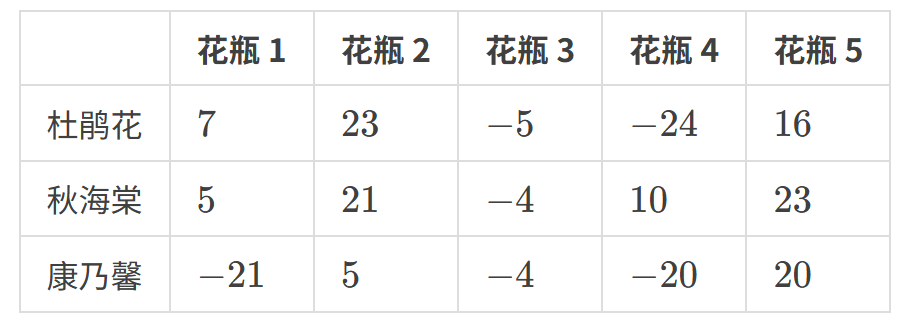
\includegraphics[scale=0.8]{images/3-1.png}
			\caption{P1854}
			\label{fig3-1}
		\end{center}
	\end{figure}
	
	根据表格，杜鹃花放在花瓶 2 中，会显得非常好看，但若放在花瓶 4 中，则显得很难看。
	
	为了取得最佳的美学效果，必须在保持花束顺序的前提下，使花的摆放取得最大的美学值。每个花束都必须被放入花瓶。 如果具有最大美学值的摆放方式不止一种，则输出任何一种方案即可。
	\subsection{题目分析}
	本题要求将 F 束不同品种的花（必须按 1~F 的严格顺序）分配到 V 个花瓶 中，每个花瓶最多放一束花，且必须全部使用这 F 束花，同时保持花的相对顺序不变（即花 i 必须放在花 j 的左边，i < j）。
	每个花瓶 j 放置花 i 会产生一个美学值 a[i][j]（可正可负可零），空瓶美学值为 0。目标是求出最大总美学值，并输出其中一种最优放置方案（花瓶编号序列）。
	约束条件：
	
	1 ≤ F ≤ V ≤ 100
	花的顺序必须严格保持（这意味着放置位置是严格递增的）
	每个花瓶至多放一朵花（但可以有空瓶）
	
	这是一个典型的带顺序约束的分配问题，可以建模为：
	
	从 V 个位置中选出 F 个位置 p1 < p2 < ... < pF
	将花 1~F 依次放入 p1~pF
	最大化 ∑ a[i][p\_i]
	
	由于 F 和 V 均 ≤ 100，直接枚举所有组合 C(V,F) 会过大（C(100,50) ≈ 10\^29），因此我们需要使用动态规划优化题目。
	\subsection{算法设计}
	定义状态：
	
	dp[i][j] 表示前 i 朵花（1~i）全部放置完毕，且最后一朵花（第 i 朵）放在第 j 个花瓶时，能达到的最大美学值总和。
	
	状态转移：
	
	
	textdp[i][j] = max{ dp[i-1][k] + a[i][j] }    (其中 1 ≤ k < j)
	
	即：第 i 朵花放在 j 号瓶，前 i-1 朵花的最后一朵放在 k 号瓶（k < j），然后加上当前放置的价值 a[i][j]。
	边界：
	
	dp[0][j] = 0  （没有花时，任何位置都是 0）
	dp[i][j] 初始为极小值（表示不可达）
	
	最终答案：
	
	max(dp[F][j])  对所有 j = F..V 取最大值（因为至少需要 F 个瓶子，且最后一朵花可以放在任意 >=F 的位置）
	
	方案记录：
	
	使用 pre[i][j] 记录 dp[i][j] 是从哪个 k 转移来的
	最后从 dp[F][best\_j] 开始回溯，依次得到放置位置
	
	\begin{lstlisting}[style=commonCodeStyle, caption={P1854.cpp}, label={lst:3-1}]
		#include<bits/stdc++.h>
		using namespace std;
		#define ll long long
		const int N=105;
		int v[N][N];
		int dp[N][N];//j瓶放到第i朵
		int n,m;
		int a,b,c;
		int pre[N][N];
		void print(int k,int pl){
			if(k==0) return;
			print(k-1,pre[k][pl]);
			printf("%d ",pl);
		}
		int main(){
			scanf("%d%d",&n,&m);
			for(int i=1;i<=n;i++){
				dp[i][0]=-2e9;
				for(int j=1;j<=m;j++) scanf("%d",&v[i][j]),dp[i][j]=-2e9;
			}
			for(int j=0;j<=m;j++) dp[0][j]=0;
			for(int j=1;j<=m;j++){
				for(int i=1;i<=n;i++){
					for(int k=i-1;k<j;k++){
						if(dp[i][j]<dp[i-1][k]+v[i][j]){
							dp[i][j]=dp[i-1][k]+v[i][j];
							pre[i][j]=k;
						}
					}
				}
			}
			int ans=-2e9,pl;
			for(int j=1;j<=m;j++){
				if(ans<dp[n][j]){
					ans=dp[n][j];pl=j;
				}
			}
			printf("%d\n",ans);
			print(n,pl);
			return 0;
		}
		/*
		3 5
		7 23 -5 -24 16
		5 21 -4 10 23
		-21 5 -4 -20 20
		*/
		//轮着来，从1束花开始
	\end{lstlisting}
	
	
	\subsection{性能分析}
	时间复杂度：O(F · V²)
	
	F,V ≤ 100，最坏情况约 100 × 10000 = 1,000,000 次操作，常数小
	
	空间复杂度：O(F · V)
	
	dp 和 pre 数组各约 100×100 = 10,000 个 int，总共约 80KB
	\subsection{运行测试}
	按照我们上方的思路与代码实现，我们设计如下的测试
	
	输入：
	
	3 5
	
	7 23 -5 -24 16
	
	5 21 -4 10 23
	
	-21 5 -4 -20 20
	
	输出：
	
	53
	
	2 4 5
	
	\begin{figure}[H]
		\begin{center}
			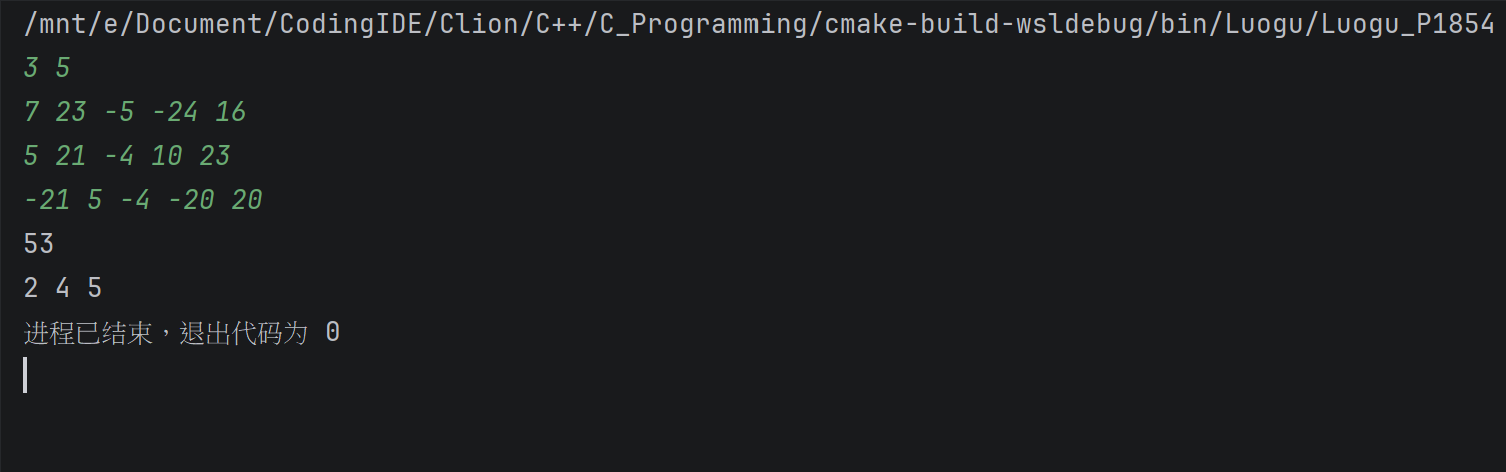
\includegraphics[scale=0.8]{images/3-2.png}
			\caption{P1854}
			\label{fig3-2}
		\end{center}
	\end{figure}
	
	\section{P1443 马的遍历}
	有一个 n×m 的棋盘，在某个点 (x,y) 上有一个马，要求你计算出马到达棋盘上任意一个点最少要走几步。
	\subsection{题目分析}
	本题要求计算在一个 n × m 的棋盘上，从起始位置 (x, y) 出发的「马」（国际象棋中的「马」），到达棋盘上每一个格子所需的最少步数。如果某个格子无法到达，则输出 -1。
	马的走法为「日」字形跳跃，即每次移动的位移为以下 8 种之一：
	
	(±1, ±2)
	(±2, ±1)
	
	题目特点：
	
	棋盘规模：1 ≤ n, m ≤ 400
	
	起点坐标：1 ≤ x ≤ n, 1 ≤ y ≤ m
	
	输出要求：完整输出 n 行 m 列的矩阵，每个位置表示从起点到该点的最短步数（不可达为 -1）
	
	无障碍物，纯粹图论最短路问题
	
	这是一个典型的无权图单源最短路问题。
	由于每一步的权重均为 1，且图的出度固定为 8，我们适合使用 BFS（广度优先搜索） 求解。
	\subsection{算法设计}
	核心思路：将棋盘上的每个格子视为图的一个节点，相邻关系由马的 8 种走法决定，使用 BFS 从起点开始进行层序遍历，记录到达每个节点的最短距离。
	
	具体实现步骤：
	
	读入棋盘大小 n, m 及起点 (sx, sy)（注意题目中 x 是行，y 是列，均从 1 开始计数）
	
	定义马的 8 个移动方向（dx[], dy[] 数组）
	
	使用二维数组 dist[][] 记录到达 (i,j) 的最少步数，初始全部置为 -1
	
	使用 vis[][] 标记是否已经访问过（避免重复入队）
	
	使用队列进行 BFS：
	
	起点入队，dist[sx][sy] = 0，vis[sx][sy] = true
	
	每次从队首取出节点，枚举 8 个方向
	
	若新位置合法（在棋盘内）且未访问，则：
	
	标记已访问
	
	距离 = 当前距离 + 1
	
	入队
	
	BFS 结束后，dist[][] 即为答案矩阵
	
	按行输出，每个数值占固定宽度（题目接受任意合理场宽，常用 %-5d 左对齐输出）
	
	代码中采用了 struct Node {int x, y, step;} 来储存节点信息，也可以使用 pair 或三元组，但 struct 方式清晰易读。
	
	\begin{lstlisting}[style=commonCodeStyle, caption={P1443.cpp}, label={lst:4-1}]
		#include <bits/stdc++.h>
		using namespace std;
		
		const int MAXN = 405;
		
		int n, m, sx, sy;
		int dist[MAXN][MAXN];  // 到 (i,j) 的最少步数，初始 -1
		bool vis[MAXN][MAXN];
		
		int dx[8] = { -1, -2, -2, -1, 1, 2, 2, 1 };  // 马的8个方向
		int dy[8] = { -2, -1, 1, 2, 2, 1, -1, -2 };
		
		struct Node {
			int x, y, step;
		};
		
		void bfs() {
			queue<Node> q;
			q.push({sx, sy, 0});
			vis[sx][sy] = true;
			dist[sx][sy] = 0;
			
			while (!q.empty()) {
				Node cur = q.front(); q.pop();
				int x = cur.x, y = cur.y, step = cur.step;
				
				for (int i = 0; i < 8; i++) {
					int nx = x + dx[i];
					int ny = y + dy[i];
					if (nx >= 1 && nx <= n && ny >= 1 && ny <= m && !vis[nx][ny]) {
						vis[nx][ny] = true;
						dist[nx][ny] = step + 1;
						q.push({nx, ny, step + 1});
					}
				}
			}
		}
		
		int main() {
			scanf("%d%d%d%d", &n, &m, &sx, &sy);
			
			memset(dist, -1, sizeof(dist));
			memset(vis, 0, sizeof(vis));
			
			bfs();
			
			for (int i = 1; i <= n; i++) {
				for (int j = 1; j <= m; j++) {
					printf("%-5d", dist[i][j]);  // 左对齐，宽5格，美观输出
				}
				printf("\n");
			}
			
			return 0;
		}
	\end{lstlisting}
	
	\subsection{性能分析}
	时间复杂度：
	
	节点数：n × m ≤ 400 × 400 = 160,000
	
	每节点出边数：固定 8
	BFS 总时间：O(节点数 + 边数) = O(n·m + 8·n·m) = O(n·m)
	最坏情况 ≈ 160,000 次操作，常数极小
	
	空间复杂度：
	
	队列最坏情况储存所有节点 ≈ 160,000 个 Node（每个约 12–16 字节） ≈ 2–3 MB
	
	总空间远低于常见限制（通常 256 MB）
	
	结论：时间与空间均为线性级别，对于 n,m ≤ 400 完全高效。
	
	\subsection{运行测试}
	输入：
	
	3 3 1 1
	
	输出：
	
	0  3  2
	
	3 -1  1
	
	2  1  4
	
	\begin{figure}[H]
		\begin{center}
			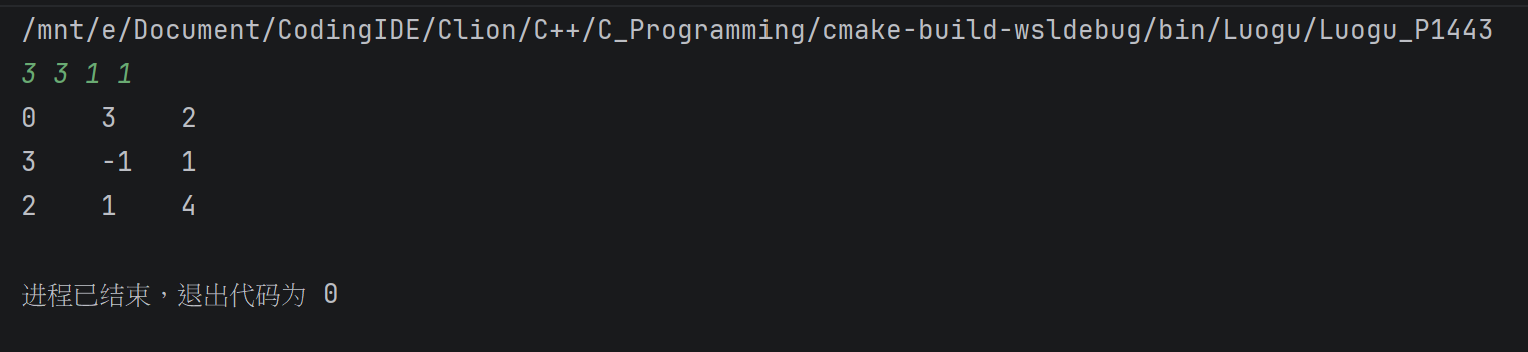
\includegraphics[scale=0.8]{images/4-1.png}
			\caption{P1443}
			\label{fig4-1}
		\end{center}
	\end{figure}
	
	\section{P1250 种树}
	路边的地区被分割成块，并被编号成 1,2,…,n。每个部分为一个单位尺寸大小并最多可种一棵树。
	
	每个居民都想在门前种些树，并指定了三个号码 b，e，t。这三个数表示该居民想在地区 b 和 e 之间（包括 b 和 e）种至少 t 棵树。
	
	居民们想种树的各自区域可以交叉。你的任务是求出能满足所有要求的最少的树的数量。
	
	\subsection{题目分析}
	本题要求在 1 到 n 的 n 个连续地块上种树，每块地最多种一棵树。有 h 个居民，每个居民提出一个区间 [b\_i, e\_i] 并要求在该区间内至少种 t\_i 棵树。所有要求必须同时满足，求最少需要种多少棵树。
	
	题目特点：
	
	每个地块至多种一棵树 → 种树位置互斥，而区间要求是「至少」而非「恰好」，即多个区间要求可以重迭，我们目标是最小化总种树数量（即最大化「空地」数量）
	
	这是一个经典的区间覆盖 + 贪心问题。
	
	核心矛盾在于：当多个区间重迭时，如何分配有限的种树位置，才能用最少的树满足所有「至少」要求。
	
	暴力枚举每个区间的具体种树位置组合不可行（h ≤ 5000，n ≤ 3e4，组合爆炸）。
	
	因此，需要找到一种贪心策略，在保证满足所有约束的前提下尽量少种树。
	
	\subsection{算法设计}
	采用从右往左扫描 + 贪心 维护已种树位置的策略。
	
	具体思路：
	
	将所有居民的要求按左端点 b\_i 从大到小排序（即从右往左处理）
	
	对每个要求 [l, r] 至少种 cnt 棵树：
	
	先查询当前 [l, r] 区间内已经种了多少棵树（sum）
	
	如果 sum ≥ cnt，则该要求已经被之前的种树满足，无需再种
	
	如果 sum < cnt，还需要再种 (cnt - sum) 棵
	
	贪心选择：在 [l, r] 内最靠右的、尚未种树的位置依次种上（因为右边位置对后续左边的要求影响较小）
	
	为了快速实现「查询区间已种树数」和「找到区间内第 k 个空位」两个操作，使用带懒目标线段树：
	
	维护每个位置的状态：0（未种）/ 1（已种）
	
	支持区间赋值（种一片树）
	
	支持区间求和（已种数量）
	
	支持查询「全局第 k 个 0」（即第 k 个空位的位置）
	
	代码实现细节：
	
	线段树 sum[x] 表示子树范围内已种树的数量
	
	tag[x] 用于懒标区间赋值（全部种或全部不种，但本题只用赋值为 1）
	
	kth0(x, k, l, r)：在当前子树中找到第 k 个 0 的位置（递归判断左子树 0 的个数）
	
	ser(x, a, b, v)：区间 [a,b] 赋值为 v（本题 v=1）
	
	\begin{lstlisting}[style=commonCodeStyle, caption={P1250.cpp}, label={lst:5-1}]
		#include<bits/stdc++.h>
		#define N 30010
		#define H 5010
		using namespace std;
		int n,h,ans;
		struct SEG{
			#define lc (x<<1)
			#define rc (x<<1|1)
			int sum[N<<2],tag[N<<2];
			void pushup(int x){sum[x]=sum[lc]+sum[rc];}
			void pushdown(int x,int l,int r){
				if(!tag[x]) return;
				int mid=(l+r)>>1;
				sum[lc]=(mid-l+1)*tag[x],sum[rc]=(r-mid)*tag[x];
				tag[lc]=tag[rc]=tag[x],tag[x]=0;
			}
			int kth0(int x,int k,int l,int r){
				if(l==r) return l;
				pushdown(x,l,r);
				int mid=(l+r)>>1,lef0=mid-l+1-sum[lc];
				if(lef0>=k) return kth0(lc,k,l,mid);
				else return kth0(rc,k-lef0,mid+1,r);
			}
			void ser(int x,int a,int b,int v,int l,int r){
				if(a<=l&&r<=b) return tag[x]=v,sum[x]=(r-l+1)*v,void();
				pushdown(x,l,r);
				int mid=(l+r)>>1;
				if(a<=mid) ser(lc,a,b,v,l,mid);
				if(b>mid) ser(rc,a,b,v,mid+1,r);
				pushup(x);
			}
			int query(int x,int a,int b,int l,int r){
				if(a>b) return 0;
				if(a<=l&&r<=b) return sum[x];
				pushdown(x,l,r);
				int mid=(l+r)>>1,ans=0;
				if(a<=mid) ans+=query(lc,a,b,l,mid);
				if(b>mid) ans+=query(rc,a,b,mid+1,r);
				return ans;
			}
		}tr;
		struct Seg{int l,r,cnt;}a[H];
		int main(){
			cin>>n>>h;
			for(int i=1;i<=h;i++) cin>>a[i].l>>a[i].r>>a[i].cnt;
			sort(a+1,a+1+h,[](Seg a,Seg b){return a.l>b.l;});
			for(int i=1;i<=h;i++){
				int sum=tr.query(1,a[i].l,a[i].r,1,n);
				if(sum<a[i].cnt){
					ans+=a[i].cnt-sum;
					int pos=tr.kth0(1,a[i].cnt-sum+a[i].l-1,1,n);
					tr.ser(1,a[i].l,pos,1,1,n);
				}
			}
			cout<<ans<<"\n";
			return 0;
		}
		
		//右边往左边开始排
		//排重迭的
		//贪心
	\end{lstlisting}
	
	\subsection{性能分析}
	时间复杂度：
	
	排序 h 个要求：O(h log h)
	
	对每个要求：
	
	查询 [l,r] 已种数：O(log n)
	
	若需补种 k 棵：每次调用 kth0 找位置 O(log n)，然后单点/区间更新 O(log n)
	
	最坏情况每个要求都补种，且每次补 1 棵 → 总更新次数 ≤ n
	
	总时间：O((h + n) log n)
	
	n ≤ 3e4，h ≤ 5e3，log n ≈ 15，总操作量 ≈ 10\^5 ~ 10\^6 级别，高效
	
	空间复杂度：
	
	线段树：4 × 30010 × sizeof(int) ≈ 480 KB
	
	要求数组：O(h) ≈ 20 KB
	
	总空间远低于限制
	
	\subsection{运行测试}
	输入
	
	9
	
	4
	
	1 4 2
	
	1 4 2
	
	4 6 2
	
	8 9 2
	
	3 5 2
	
	输出
	
	5
	
	\begin{figure}[H]
		\begin{center}
			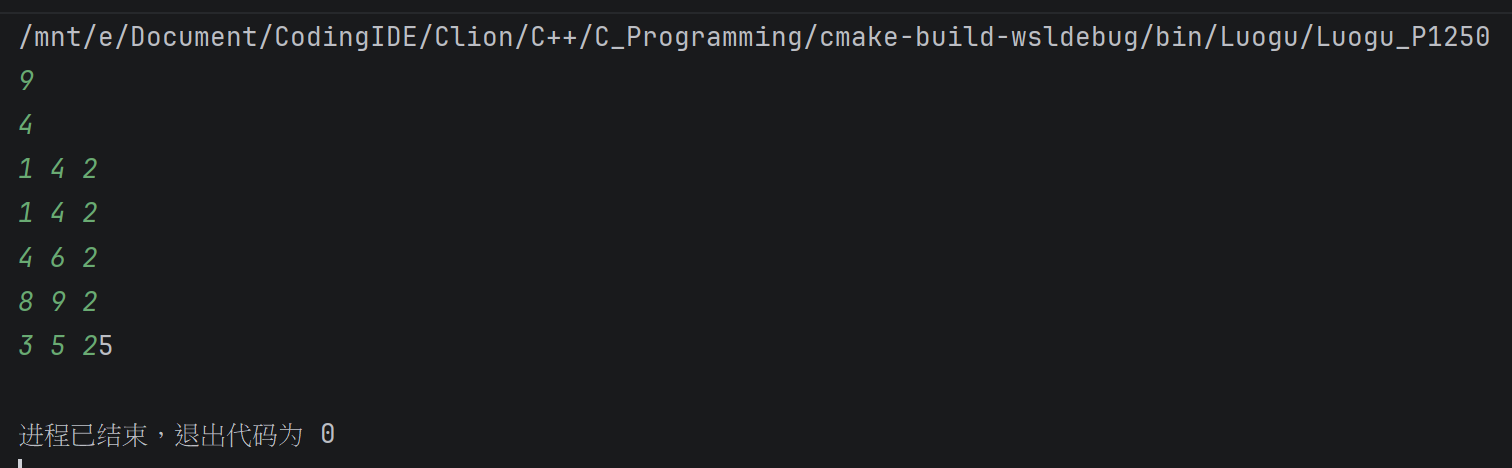
\includegraphics[scale=0.8]{images/5-1.png}
			\caption{P1250}
			\label{fig5-1}
		\end{center}
	\end{figure}
	
	\section{P1111 修复公路}
	给出 A 地区的村庄数 N，和公路数 M，公路是双向的。并告诉你每条公路的连着哪两个村庄，并告诉你什么时候能修完这条公路。问最早什么时候任意两个村庄能够通车，即最早什么时候任意两条村庄都存在至少一条修复完成的道路（可以由多条公路连成一条道路）。
	
	\subsection{题目分析}
	本题描述地震后所有公路损坏，给出 N 个村庄、M 条双向公路，每条公路有修复完成时间 t。问最早什么时候使得任意两个村庄都能通过已修复完成的公路（可经过多条）互相连通，即整个图连通的最早时刻。如果即使所有公路修好后仍不连通，输出 -1。
	
	题目核心：
	
	每条公路有不同的修复完成时间 t
	
	时间 t 时，所有 t' ≤ t 的公路都已修好，可通行
	
	要求整个图（N 个点）在某个时刻变成单连通分量
	
	输出这个时刻的最小值（即最后一条使图连通的公路的 t）
	
	所以我们知道这就是一个经典的最小生成树 + 边按权重排序的应用场景，但权重不是成本，而是时间，且我们关心的是「使连通分量数从 N 减到 1 的最后一条边的时间」。
	\subsection{算法设计}
	采用 Kruskal 算法 的变形，按修复时间从小到大排序边，逐步加入已修复的公路，并使用并查集维护连通分量。
	
	读入 N（村庄数）、M（公路数）
	
	读入 M 条公路：x, y, t（连接 x 和 y，修复完成时间 t）
	
	将所有公路按 t 升序排序（从最早修好到最晚修好）
	
	初始化并查集：每个村庄独立，连通分量数 = N
	
	依次遍历排序后的公路：
	
	若两端点 x 和 y 不在同一连通分量（find(x) ≠ find(y)）
	
	合并它们（union）
	
	连通分量数减 1
	
	每次合并后检查：若连通分量数 == 1，则当前公路的 t 就是答案（因为这条公路是最后一条使图连通的边）
	
	若遍历完所有边后连通分量仍 > 1，输出 -1
	
	\begin{lstlisting}[style=commonCodeStyle, caption={P1111.cpp}, label={lst:6-1}]
		#include <bits/stdc++.h>
		using namespace std;
		int father[1005];
		struct road
		{
			int x;
			int y;
			int t;
		}r[100005];
		int cmp(road x,road y)
		{
			return x.t<y.t;
		}
		int find(int x)
		{
			if(father[x]==x) return x;
			else return find(father[x]);
		}
		void union_set(int x,int y)
		{
			int fx=find(x);
			int fy=find(y);
			father[fy]=fx;
		}
		int main()
		{
			int n,m;
			cin>>n>>m;
			for(int i=1;i<=n;i++)
			{
				father[i]=i;
			}
			for(int i=1;i<=m;i++)
			{
				cin>>r[i].x>>r[i].y>>r[i].t;
			}
			sort(r+1,r+1+m,cmp);
			for(int i=1;i<=m;i++)
			{
				if(find(r[i].x)!=find(r[i].y)) 
				{
					union_set(r[i].x,r[i].y);
					n--;
				}
				if(n==1)
				{
					cout<<r[i].t;
					return 0;
				}
			}
			cout<<"-1";
			return 0;
		}
		
		//应从最快的开始修
		//修一次就检查一次是否全部连通
		//通了就合并
		
	\end{lstlisting}
	
	\subsection{性能分析}
	时间复杂度：
	
	读入 + 排序 M 条边：O(M log M)
	
	并查集操作：
	
	总共 M 次 find + 最多 N-1 次 union
	
	使用路径压缩 + 按秩合并（或本题简单实现的路径压缩）后，近似 O(M α(N))，α(N) ≈ 4
	
	N ≤ 1000，M ≤ 10\^5，总时间 ≈ O(M log M) 主导，远低于 1 秒
	
	空间复杂度：
	并查集 father[]：O(N) ≈ 4 KB
	
	总空间极小
	
	\subsection{运行测试}
	4 4
	1 2 6
	1 3 4
	1 4 5
	4 2 3
	
	\begin{figure}[H]
		\begin{center}
			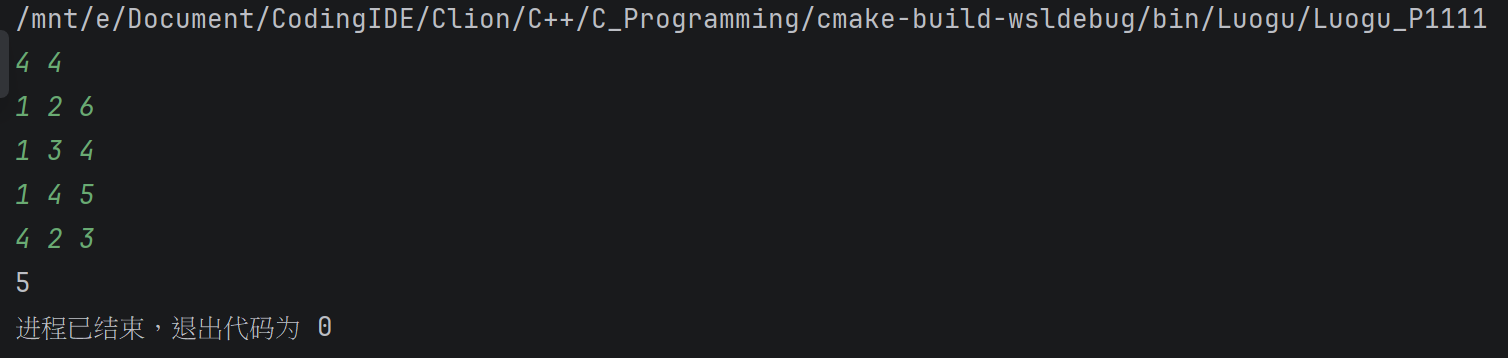
\includegraphics[scale=0.8]{images/6-1.png}
			\caption{P1111}
			\label{fig6-1}
		\end{center}
	\end{figure}
	
	\section{总结}
	通过《算法设计与分析》实验课上的实践，我完成了多类经典算法题目的编码、调试与优化过程，了解到不同的算法思想和数据结构
	
	分治法
	
	相关题目：洛谷 P1228 地毯填补（缺陷棋盘 L-三连覆盖）
	
	利用问题的自相似性，将大规模问题分解为四个子问题，并在每次分解时「人为制造缺陷」来保持递归不变性；熟练掌握二维坐目标象限判断与中心点放置策略。
	
	动态规划
	
	相关题目：P1854 [IOI1999] 花店橱窗布置
	
	处理带严格顺序约束的分配问题时，如何定义「前 i 个物品放到第 j 个位置」的状态；掌握二维 DP + 前驱记录回溯路径的标准写法；理解负数价值时初始化为极小值的必要性。
	
	图论搜索（BFS）
	
	相关题目：P1443 马的遍历
	
	将棋盘模型化为图，使用 BFS 求单源最短路；熟练处理八方向移动的坐标偏移；掌握二维 vis 数组与 dist 数组的配合使用，以及输出格式的对齐技巧。
	
	贪心 + 线段树优化
	
	相关题目：P1250 种树
	
	从右往左扫描的贪心策略在「区间至少覆盖」问题中的正确性；线段树支持「区间赋值」「区间求和」「查询第 k 个 0」三种操作的综合应用；理解如何用数据结构弥补纯贪心难以精确定位的缺陷。
	
	并查集 + Kruskal 变形
	
	相关题目：P11111 修复公路
	
	将「最小生成树」思想应用到「最早连通时间」问题；按时间排序后逐步加入边，并实时维护连通分量数的技巧；理解「最后一条使连通分量数从 N 变为 1 的边的权重」即为答案。
	
	通过这学期的算法实践，我深刻感受到算法学习的核心关键，而在于理解每种范式的本质以及面对新问题时的建模能力。从最开始写暴力解法 TLE，到后来逐步学会分析数据范围、选择合适算法、优化时间复杂度，这整个过程让我对「如何思考算法题」有了更系统的认识。
	
	
	
	
	
\end{document}
